%%%%%%%%%%%%%%%%%% Część I %%%%%%%%%%%%%%%%%

\section{Generowanie drzew decyzyjnych}

\subsection{Generowanie drzewa}

\begin{itemize}
\item \textbf{Obejrzyj zawartość plików \emph{golf.nam}, \emph{golf.dat} i~\emph{golf.tst}; ile przykładów zawiera zbiór uczący? Iloma atrybutami są~one opisane?}
	\\Zbiór uczący zawiera 14 przykładów. Są one opisane pięcioma atrybutami, w tym jednym atrybutem decyzyjnym.

\item \textbf{Wygeneruj drzewo dla zbioru przykładów \emph{golf}; ustawienia standardowe.}

Drzewo przed pruningiem:	 
	\begin{verbatim}
outlook = overcast: Play (4.0)
outlook = sunny:
|   humidity <= 75 : Play (2.0)
|   humidity > 75 : Don't Play (3.0)
outlook = rain:
|   windy = true: Don't Play (2.0)
|   windy = false: Play (3.0)
	\end{verbatim}
	
Drzewo po pruningu:
	\begin{verbatim}
outlook = overcast: Play (4.0/1.2)
outlook = sunny:
|   humidity <= 75 : Play (2.0/1.0)
|   humidity > 75 : Don't Play (3.0/1.1)
outlook = rain:
|   windy = true: Don't Play (2.0/1.0)
|   windy = false: Play (3.0/1.1)
	\end{verbatim}





\item \textbf{Przeanalizuj wyniki; czy udało się przeprowadzić pruning?}
	\\Nie udało się przeprowadzić pruningu. Drzewa są identyczne.

\item \textbf{Obejrzyj drzewo; ile ma węzłów decyzyjnych, a~ile liści?}
	\\Wygenerowane drzewo ma 3 węzły decyzyjne i 5 liści.

\item \textbf{ Prześledź ścieżkę od korzenia do wybranego liścia.}
		\\W korzeniu znajduje się test związany z atrybutem outlook. Jeśli dla klasyfikowanego przykładu wartość atrybutu outlook wynosi "sunny", to następny węzeł na ścieżce to ten związany z atrybutem humidity. Zakłądając, że dla omawianego przykładu wilgotność jest większ niż $ 75\% $ , liściem w analizowanej ścieżce będzie liść odnoszący się decyzji "Don't Play".
		\\Inaczej mówiąc, ścieżk ta klasyfikuje wszystkie dni w które jest słoneczna pogoda i wilgotność większa niż $ 75\% $ jako dni, w które nie gra się w golfa.
		
\item \textbf{Porównaj estymaty błędu dla drzewa oryginalnego (\emph{Unpruned}) i~uproszczonego (\emph{Pruned}).}
	\\Estymata błędu dla oryginalnego drzewa wynosi  $ 0\% $ a dla uproszczonego $ 38,5\% $ .

\item \textbf{Obejrzyj macierz pomyłek.}
	\\Ponieważ drzewo oryginalne nie generuje błędów dla zbioru uczącego, to też jedyne co można z niego odczytać, to właśnie, że żadne obiekty nie są błędnie klasyfikowane, oraz że w przypadku 9 przykładów drzewo poprawnie zaklasyfikowało przykłady do klasy "Play" a w 5 przypadkach do klasy "Don't Play".

\end{itemize}

\subsection{Konsultowanie}

\begin{itemize}
\item Dokonaj konsultacji wymyślonego przykładu dla wygenerowanego drzewa.
	\\Dokonano konsultacji przykładu o wartościach atrybutów: outlook = overcast, temperature = 5, humidity = 100, windy = true. W wyniku konsultacji podanego przykładu otrzymano decyzję "Play". Poneważ wartości atrybutów zostały podane w sposób deterministyczny to decyzja ta była pewna (prawdopodobieństwo, że analizowany przykład należy do klasy "Play" wynosiło 1). Wynik jest zgodny z oczekiwaniami, poniważ wygenerowane drzewo decyzyjne na podstawi galęzi "Outlook = overcast" przydziela wszystkie przykłady z taką wartością atrybutu do klasy "Don't play", niezależnie od wartości pozostałych atrybutów.
	
\item Konsultowanie przykładu ,,niepełnego''; dokładnie przeanalizuj wynik.
	\\Przykład niepełny miał postać: (overcast = sunny, temperature = 15, humidity = ?, windy = false). Przechodząc ścieżkę klasyfikującą ten przykład dochodzimy do atrybutu humidity. Nie jest znana wartość analizowanego przykładu na tym atrybucie, więc zostają obliczone prawdopodobieństwa przyjęcia konkretnych wartości. W analizowanym węźle (za gałęzią "sunny") znajduje się 5 przykładów uczących, w tym 2 ( $ 40\% $ ) przyjmują wartość "humidity" większą niż $ 75\% $ a 3  $ ( 60\% ) $ mniejszą. Dlatego przyjmuje się, że analizowany przykład będzie miał z prawdopodobieństwem $ 60\% $ wartość humidity większą niż $ 75\% $ a mniejszą z prawdopodobieństwem $ 40\% $ .	Dalej w drzewie sa juz tylko liście, można więc obliczyć rpawdopodobieństwo całych kompletów wartości: z prawdopodobieństwem $ 40\% $ analizowany przykład przyjmie wartości (overcast = sunny, temperature = 15, humidity  $ > 75\% $, windy = false) a z prawdopodobieństwem $ 60\% $ wartości  (overcast = sunny, temperature = 15, humidity $ >  75\% $ , windy = false). Drugie prawdopodobieństwo jest wyższe, więc z prawdopodobieństwem $ 60\% $ konsultowany przykład zostaje przypisany do klasy "Don't Play"
	
\item Konsultowanie, gdy znany jest rozkład prawdopodobieństwa.
	\\W przypadku przykładu ze znanym rozkładem prawdopodobieństwa analizowane są wszystkie gałęzie o niezerowym prawdopodobieństwie z wagami odpowiadającymi przypisanym danm wartośćiom prawdopodobieństwom. Analizowany przykład miał postać: P(sunny) = $ 0.8 $ , P(overcast) = $ 0.2 $ . Dlatego, jeśli wartość humidity była większa niż $ 75\% $ to algorytm przydzielał przykład z $ 20\% $ prawdopodobieństwem do klasy "Play" i $ 80 \% $ prawdopodobieństwem do klasy "Don't play". Ponieważ dla "humidity" mniejszej niż $ 75\% $ i "outlook" = "sunny" drzewo podejmuje decyzję "Play", taką samą jak przy "outlook" = "overcast", to prtawdopodobieństwa wtedy się sumują i lagorytm podejmuje decyzję "Play" z prawdopodobieństwem $ 100 \% $ .

\end{itemize}

\subsection{Różnica między \emph{gain ratio} a~\emph{info gain} w~praktyce}

\begin{itemize}
\item Obejrzyj zbiór \emph{testgain} (\emph{dat} i~\emph{nam}).
\item Wygeneruj dla niego dwukrotnie drzewo z~użyciem opcji \emph{gain ratio} i~\emph{info gain}; skomentuj wyniki.
	\\

	Drzewo wygenerowane z użyciem opcji InfoGain:		
		\begin{verbatim}
			a1 = 1: A (2.0)
			a1 = 2: A (2.0)
			a1 = 3: B (2.0)
			a1 = 4: B (2.0)	
		\end{verbatim}


	Drzewo wygenerowane z użyciem opcji GainRatio:
		\begin{verbatim}
			a2 = 1: A (4.0)
			a2 = 2: B (4.0)
		\end{verbatim}

	Oba atrybuty są typu wyliczeniowego (pzyjmują wartości z określonego w definicji problemu zbioru). Zbiór wartości atrybutu a1 ma wielkość 4 a atrybutu a2 wielkość 2. Współczynnik InfoGain dla obu atrybutów wynosi 1, nie preferuje więc atrybutu a2, którego dziedzina ma mniej  wartości niż dziedzina atrybutu a1. Inaczej jest w przypadku współczynnika GainRatio:  preferuje on atrybuty o mniejszych dziedzinach. Współczynnik ten wynosi $ 1/2  $ dla atrybutu a1 i $ 1 $ dla atrybytu a2, co za tym idzie w drzewie zbudowanym przy jego pomocy brany jest pod uwagę atrybut a2. Jak widać wpływa to pozytywnie na rozmiar drzewa a co za tym idzie jego prostotę i łatwość interpretacji.

	
\end{itemize}

\subsection{Grupowanie wartości atrybutów}

\begin{itemize}
\item Wygeneruj drzewo dla zbioru \emph{testgain}, zaznaczając opcję \emph{Subsetting}.
	\begin{verbatim}
	a1 in {1,2}: A (4.0)
	a1 in {3,4}: B (4.0)
	\end{verbatim}
Jak widać grupowanie wpłynęło pozytywnie na wielkość generowanego drzewa.

\item Analogicznie dla \emph{CRX}: opisać problem (przyznawanie kard kretytowych), obejrzeć zbiór (atrybuty \emph{A4}, \emph{A6} i~\emph{A7} mają wiele wartości); wygenerować drzewo bez i~z~grupowaniem.
\\Ponieważ dane dotyczące tego problemu zawierały poufne dane etykiety atrybutów zostały zmienione na nie nieznaczące symbole.
\\W problemie tym występują dwie klasy decyzyjne: "+" i "-". W zbiorze uczącym mogą mieć one interpretację klientów, którzy odpowiednio: spłacali lub niespłacali zaciągniętych kredytów w terminie spłaty. Przy klasyfikacji mogą mieć one interpretację: pozytywne lub negatywne rozpatrzenie wniosku o przyznanie karty kredytowej.
Każdy klient opisany jest za pomocą 15 atrybutóW, w tym 6 atrybutów przyjmujących wartości ciągłe i 9 atrybutów przyjmujących wartości ze znanych 2 do 14 elementowych zbiorów.



\item Obejrzeć macierz pomyłek dla zbioru uczącego i~testującego; czy w~tym zastosowaniu przydałaby się macierz kosztów pomyłek?
\\Dla drzewa bez grupowania procent błędnych klasyfikacji w zbiorze trenującym wynosi $ 6,5\% $, w zbiorze testowym $20,5\%$.
\\Dla drzewa z grupowaniem wartości te wynoszą odpowiednio $6,7\%$ i $17,5\%$. Na podstawie tych wartości można się domyślać, że występuje zjawisko przeuczenia: dla większego drzewa 
(bez grupowania) różnica w trafność klasyfikacji przykładów ze zbioru uczącego i testowego jest większa niż dla mniejszego drzewa.
\\To czy warto wprowadzić macierz kosztów pomyłek zależy od analiz ekonomicznych banku - może okazać się, że mniejszą stratę przynosi wydanie karty "złemu" klientowi niż niewydanie karty "dobremu" klientowi - np. klient niespłącający w terminie może być wbrew pozorom zjawiskiem korzystnym, ponieważ jeśli w końcu zapłaci karne odsetki to mogą one stanowić dla banku dodatkowy zysk, większy niż koszty obsługi kredytu. Zgodnie z wiedzą banku macierz kosztów pomyłek powinna być skonstruowana tak, żeby minimalizować błędy pierwszego (false positive) lub drugiego (false negative) rodzaju, w zależności od tego które z nich są dla banku bardziej kosztowne.

\end{itemize}

\subsection{Poszukiwanie optymalnej wielkości drzewa uproszczonego}

\begin{itemize}
\item Poszukiwanie optymalnej wielkości drzewa uproszczonego przez dobór poziomu ufności procedury upraszczającej (\emph{Pruning confidence level}); przeprowadź serię eksperymentów \emph{10-fold cross-validation} dla zbioru \emph{Monk2}, ze~zmieniającym się poziomem ufności od~0.05 do~0.5, z~krokiem co najwyżej 0.05. Sporządź wykres zależności:

\begin{itemize}
	\item średniego (po \emph{cross-validation}) rozmiaru drzewa uproszczonego,  
	\item średniej trafności klasyfikowania drzewa uproszczonego na~zbiorze testującym,
	\item średniej estymaty błędu dla drzewa uproszczonego...
	\\w funkcji poziomu ufności (odnieś te wyniki do średniej charakterystyki drzewa oryginalnego, nieuproszczonego).
\end{itemize}

Zgodnie z dokumentacją programu c4.5, im mniejsza wartość parametru "Pruning confidence level" tym mniejszy rozmiar drzewa po pruningu. Widać to n wykresie \ref{p1t5-rozmiar}. Dla porównania, średnia wielkość drzewa przed pruningiem wynosiła $ 63.3 $.

Wraz ze zmniejszaniem wielkości drzewa róśnie estymata błędu klasyfikacji. Jest to zrozumiałe, ponieważ estymata jest obliczana na podstawie zbioru uczącego, a oryginalne drzewo jest do niego najlepiej dopasowane. Inaczej jest w przypadku zbioru testowego: trafność klasyfikacji przykładów z tego zbioru jext najwyższa dla Pruning confidence level = 0.2. Dla mniejszych drzew trafność maleje ponieważ są one zbyt uproszczone, dla większych, ponieważ są one przeuczone (dopasowane za bardzo do zbioru uczącego). Trafność dla drzewa nieprzyciętego jest dla wszystkich badanych rozmiarów drzewa mniejsza niż dla drzewa przyciętego - uwidacznia to przeuczenie drzewa.

Analizując otrzymane wyniki można stwierdzić, że optymalna wielkość drzewa uproszczonego to ta, którą osiąga ono dla Pruning confidence level = 0.2, czyli 17.5. Dla tej wartości trafność klasyfikacji na zbiorze testowym jest największa, jednocześnie jest to małe drzewo, niemal czterokrotnie mniejsze od drzewa oryginalnego.

\begin{figure}	
	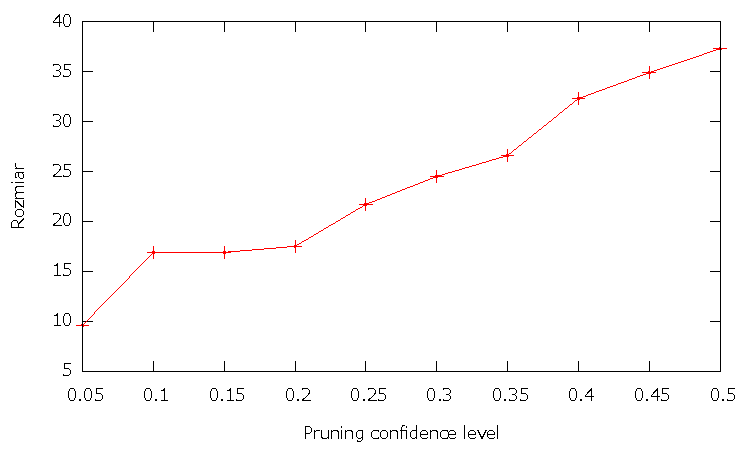
\includegraphics[scale=0.7]{figures/part1/task5/rozmiar.pdf}
	\label{p1t5-rozmiar}
	\caption{Wykres zależności średniego (po \emph{cross-validation}) rozmiaru drzewa uproszczonego w funkcji poziomu ufności. Rozmiar drzewa nieprzyciętego pokazano dla porównania, jest on niezależny od parametru "Pruning confidence level"}
\end{figure}

\begin{figure}	
	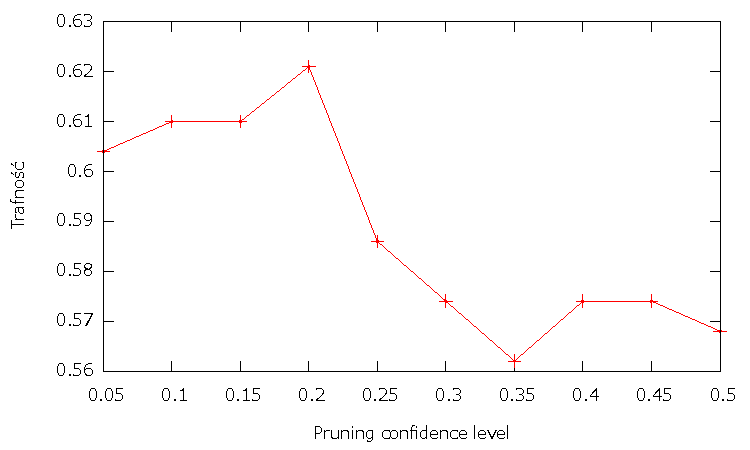
\includegraphics[scale=0.7]{figures/part1/task5/trafnosc.pdf}
	\label{p1t5-trafnosc}
	\caption{Wykres zależności średniej (po \emph{cross-validation}) trafności klasyfikacji dla drzewa uproszczonego na zbiorze tesującym w funkcji poziomu ufności. Trafność dla drzewa nieprzyciętego pokazano dla porównania, jest ona niezależna od parametru "Pruning confidence level" }
\end{figure}

\begin{figure}	
	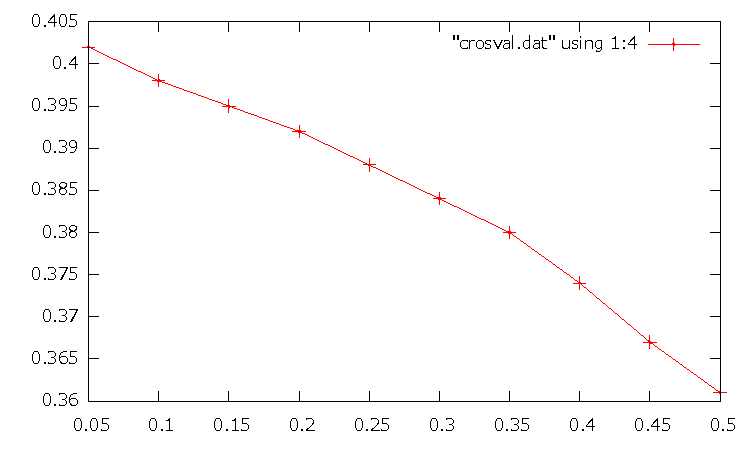
\includegraphics[scale=0.7]{figures/part1/task5/estymata.pdf}
	\label{p1t5-estymata}
	\caption{Wykres zależności średniej (po \emph{cross-validation}) estymaty błędu dla drzewa uproszczonego w funkcji poziomu ufności}
\end{figure}

\item Poszukiwanie optymalnej wielkości drzewa uproszczonego poprzez prepruning, tj.~manewrowanie minimalną licznością węzła (\emph{Minimum objects}). Dla zbioru \emph{CRX} przebadać przedział od~2 do~10.
\item Analiza wygenerowanego drzewa: poszukiwanie słabych punktów (liści o~małym wsparciu, poddrzew które generują szczególnie dużo błędów, etc.).


\end{itemize}

\subsection{\emph{Windowing}}

\begin{itemize}
\item Wyjaśnić zasadę i~opcje: \emph{Trials}, \emph{Initial window size}, \emph{Window increment}.
\item Analiza wyników (\emph{CRX}).
\end{itemize}

\subsection{Generowanie krzywej uczenia}

\begin{itemize}
\item Dla zbioru \emph{vote} przygotować kilka[naście] zbiorów uczących o~liczności $n$ zmieniającej się od~50 do~300, ze~skokiem np.~50 przypadków, poprzez wybieranie pierwszych $n$ ze~zbioru \emph{vote.dat}.
\item Wykreślić jako funkcję $n$ rozmiar drzewa uproszczonego oraz trafność klasyfikowania drzewa uproszczonego na zbiorze testującym.

\end{itemize}

\subsection{Maksymalizacja trafności}

\begin{itemize}
\item Uzyskaj jak najwyższą trafność klasyfikowania ze~zbioru \emph{GERMAN} w~eksperymencie \emph{10-fold CV}. Jakimi parametrami i~mechanizmami można manipulować, by~szukać najwyższej trafności? Kiedy można ufać tak uzyskanej trafności, a~kiedy można mówić o~nadużyciu?
\end{itemize}